\chapter{Related work}

This section will present related research findings, starting with articles
related to reinforcement learning. An overview of some related work with pose
estimation will then be discussed.

\section{Reinforcement learning for robotic manipulation}

Improvements on previous methods for Atari games using an on-policy
actor-critic method called \textit{Asynchronous Advantage Actor Critic} (A3C),
where simulation and gradient calculations were distributed on multiple cores
on a CPU, were shown to result in a reduction in training time from 8 days on
GPU to 1 day compared to original results. A stochastic actor output was
parameterized as a Gaussian distribution with mean vector $\mu$ and covariance
matrix $\sigma\mathbf{I}$. The algorithm was also successfully used on
continuous action/state-space 2D-reaching and 3D-manipulation tasks using
simulated robots \cite{mnih2016asynchronous}. Using an off-policy actor-critic
method called \textit{Deep Deterministic Policy Gradient} (DDPG)
\cite{lillicrap2015continuous}, where the actor output instead is
deterministic, solves similar tasks in simulation. This was later also shown to
be capable of learning in real-time on real robotic systems on a door opening
task \cite{gu2016deep} where data collection was distributed over a collection
of robots. The door opening task was however learned faster in the same setting
using a \textit{Normalized Advantage Functions}-algorithm (NAF) suggested by Gu
et al. \cite{gu2016continuous} where the advantage function is parameterized as
a quadratic expression, giving the Q-function estimate an easily accessible
known global maximum. Door opening tasks using NAF and DDPG used known door
poses and arm poses from attached sensor equipment as inputs.  Chebotar et al.
\cite{chebotar2016path} demonstrates door opening tasks initialized from human
demonstration using GPS and Policy Improvement with Path Integrals
($\mathbf{PI}^2$) \cite{theodorou2010generalized}. They demonstrate that they
can learn this task using pose estimation from visual input. This is extended
by Yahya et al.  \cite{yahya2016collective} to be trained simultaneously on
several robots. In both cases, torque commands were the output of a neural
network where the first part takes visual input and is pretrained with pose
estimates of the door and the robot arm. The quality of the trained policies
were evaluated when the camera position was changed by $4-5$ cm translations
and was shown to half the performance. The neural network is shown in figure
\ref{fig:gps_net}. The above methods are all summarized in table
\ref{table:algo_comparison}.

\begin{figure}[h]
    \centering
    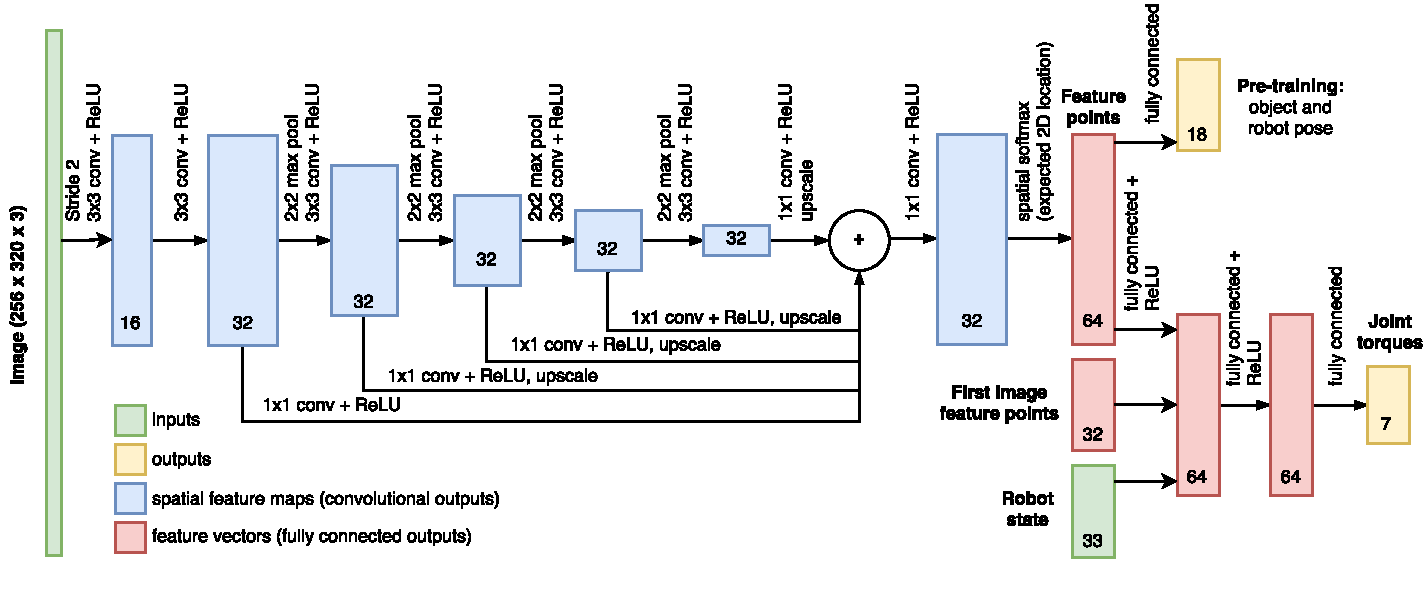
\includegraphics[width = 1.0\textwidth]{res/gps-net.pdf}
    \caption{Network used for door opening task from visual inputs \cite{chebotar2016path}}
    \label{fig:gps_net}
\end{figure}

\begin{landscape}
    \begin{table}
        \centering
        \begin{tabular}{|l|p{1.3cm}|l|p{4cm}|l|p{6cm}|}
            \hline
            \textbf{Algorithm} & \textbf{Actor/ Critic} & \textbf{-policy} & \textbf{Possible limitations} & \textbf{Deterministic} & \textbf{Empirical results} \\
            \hline
            NAF \cite{gu2016continuous} & No & Off & Quadratic advantage function & Yes & Real-world trained door opening without human demonstration where it performed better than DDPG \\
            \hline
            DDPG \cite{lillicrap2015continuous} & Yes & Off & Possibly unstable & Yes & Real-world trained door opening, no demonstration \\
            \hline
            A3C \cite{mnih2016asynchronous} & Yes & On & Uni-modal gaussian action distribution & No & Substantial speedup on training of Atari games using distributed simulations and gradient calculations, also solved continuous tasks in simulation \\
            \hline
            GPS \cite{levine2013guided} & No & Off & Uni-modal gaussian action distribution & No & Real-world trained door opening, from demonstration \\
            \hline
        \end{tabular}

    \caption{Comparison between different reinforcement learning algorithms
    used for robotic manipulation tasks.}

    \end{table}
    \label{table:algo_comparison}

\end{landscape}

\section{Pose estimation}

\subsection{Predicting poses as 2D image coordinates}

Since 2D coordinates have been shown to sufficient for 3D pose estimation
\cite{chebotar2016path}, alternative methods could include first regressing to
known 2D image coordinates as a pre-training step. Directly regressing to poses
labeled in the image have been successfully implemented by first creating
Gaussian heat-maps as targets and then regressing last layer convolution
feature maps directly to these heat-maps
\cite{newell2016stacked,tompson2014joint}. These networks were used to predict
human poses in the image frame, defined as position of joints and other key
points like the nose. The networks successfully learned not only visible parts,
but could infer parts faced away from the camera.  State-of-the-art performance
was attained by stacking several identical (regarding architecture) networks
called ''hourglass''-modules. The modules apply a series of convolutions,
followed by a series of upscalings, to output the same shape as the input.
Shortcut connections are also introduced between feature maps of the same size,
passed through $1x1$ convolutions \cite{newell2016stacked}.

\subsection{Human joint 3D relative pose prediction}

Research by Park et al \cite{park20163d} regresses 3D joint poses relative to a
root joint from images by using a convolutional neural network. The network
ends with two separate fully connected parts, one which regresses to the 2D
image coordinates of each joint, and one which regresses to the 3D relative
joint pose. They argue that by simultaneously training the network with 2D and
3D labels, this relationship is implicitly learned.

%\section{Motion planning by a predictive model}
%
%Another method for learning manipulation tasks was shown by Finn and Levine
%\cite{finn2016deep}. Given a sequence of initial images, they denote it
%$I_{0:1}$, together with robot poses $x_{0:1}$, and future commands $a_{1:H_p}$
%where $H_p$ is some prediction horizon, they predict the distribution of future
%images $I_{2:H_p + 1}$. $I_t$ is here a collection of independent pixel
%distributions with mean $\hat{I}_t$. A convolutional LSTM was used for this,
%and an implicit feature of the network is what they call a flow map
%$\hat{F}_t(x, y, k, l)$ which is the probability of the pixel at coordinates
%$(k, l)$ at time $t+1$ originating from coordinates $(x, y)$. Given a flow map
%they can do one step prediction:
%
%\begin{equation}
%    \hat{F}_t \odot \hat{I}_t := \sum_{k \in (-\kappa, \kappa)} \sum_{l \in (-\kappa, \kappa)} \hat{F}_t(x,y,k,l)\hat{I}_t(x-k, y-l) = \hat{I}_{t+1}
%\end{equation}
%
%When using these implicit flow operators rather than actual predicted image
%which was the output from the network, they can predict movement of individual
%pixels for several time steps ahead. Using a maximum likelihood approach, they
%can find the series of actions that puts a pixel at some other target location.
%For evaluation, they try their trained algorithm on previously unseen objects
%by selecting start and end coordinates for which it generalized.
%
%An interesting feature of their approach is that the data set for training was
%generated by torque-controlled arms randomly interacting with a collection of
%objects and recording images of it along with the robot poses. Therefore, no
%part of the training needed human supervision or demonstration. Another feature
%is that the camera positions were not the same across robots, it is unclear if
%they evaluated the method with a new camera position though.
%
